\section{Caracterización del sistema optimizado}
\subsection{Selectividad}\label{sec:selecresults}\index{PIM!Selectividad}
Los perfiles de transporte competitivo de ion litio contra sodio, potasio y magnesio en relaciones molares (\ce{Li+}/\ce{M^n+}) 1:1, 1:10 y 1:100 se muestran en la Figura \ref{fig:selectivity1}.

\begin{figure}[H]
    \centering
    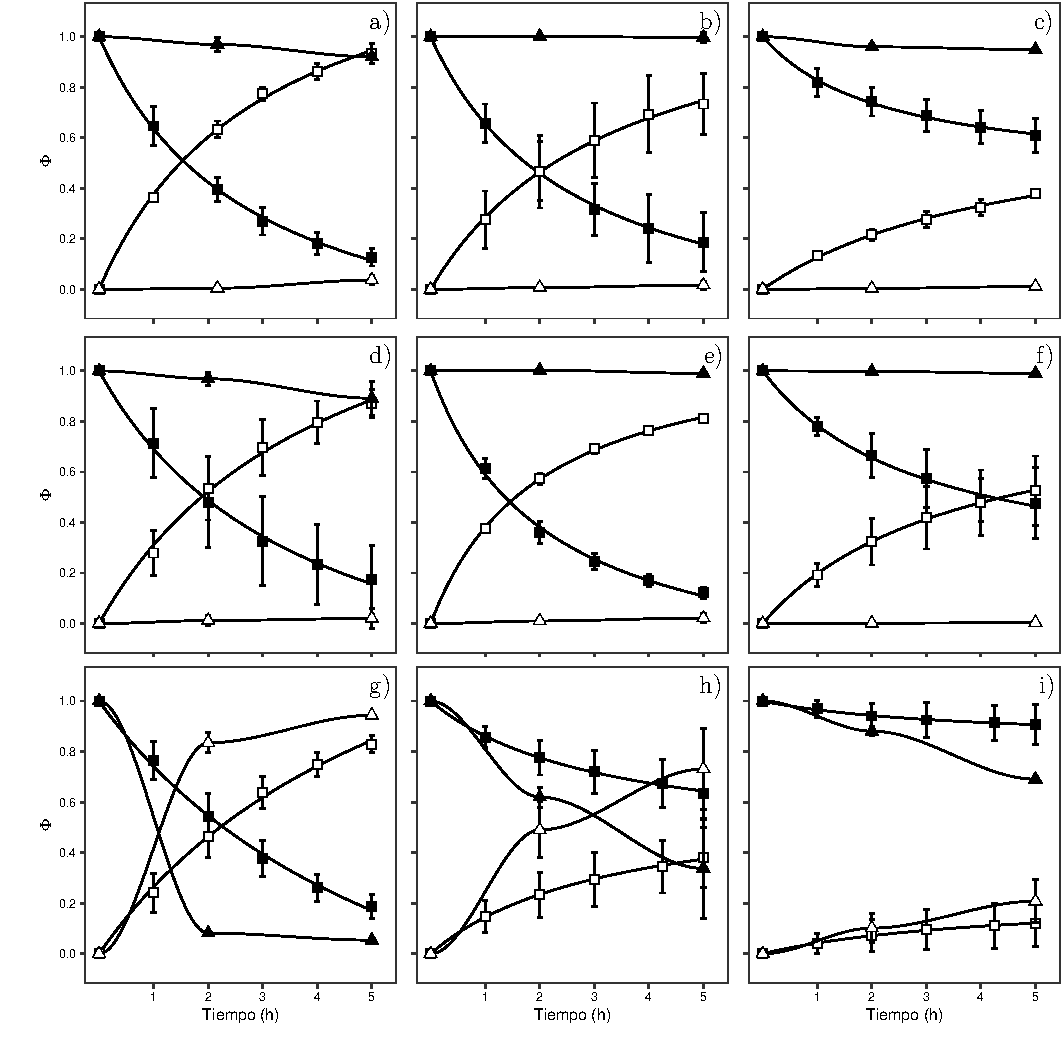
\includegraphics[width=\textwidth]{chap5/figures/thesis-selectividad.pdf}
    \caption[Perfiles de transporte competitivo de ion litio contra sodio, potasio y magnesio.]{Perfiles de transporte de ion litio en presencia de otros cationes interferentes a distintas relaciones molares: sodio 1:1 (a), sodio 1:10 (b), sodio 1:100 (c), potasio 1:1 (d), potasio 1:10 (e), potasio 1:100 (f), magnesio 1:1 (g),  magnesio 1:10 (h) y magnesio 1:100 (i). Ion litio en la fase de alimentación (\protect\squareblck), ion litio en la fase de recuperación (\protect\squarewht), catión interferente en la fase de alimentación (\protect\triangleupblck) y catión interferente en la fase de recuperación (\protect\triangleupwht).}
    \label{fig:selectivity1}
\end{figure}

\clearpage El sistema presenta buena selectividad frente a los cationes alcalinos sodio y potasio. La presencia de estos iones ocasiona una disminución considerable en la permeabilidad de la membrana frente a los iones litio. Este efecto es más marcado cuando las relaciones molares de sodio y de potasio respecto al ion litio son grandes. La fracción transportada de sodio y de potasio se mantiene baja y disminuye con el aumento en su concentración inicial en la disolución de alimentación. Esto se debe a que si la concentración de los iones en la disolución de alimentación es alta, una mayor cantidad neta debe ser transportada para observar un cambio apreciable en las fracciones de cada fase. En otros términos, esto implica que aunque la fracción transportada de sodio y potasio se mantiene baja, una cantidad apreciable de estos iones si es transportada ocupando sitios activos de la membrana y naturalmente, esto disminuye la eficiencia con la que el ion litio es extraído.

Un comportamiento muy diferente lo presenta el catión divalente magnesio que no es excluido por la PIM sino que es transportado incluso con mayor eficiencia que el ion litio. Esto se observa aún cuando su concentración molar es dos órdenes de magnitud mayor a la del ion litio. Varios autores \citep{Liu2020, Zhang2019} han atribuído la falta de selectividad hacia el magnesio por parte de varios de los sistemas destinados a la separación de ion litio al hecho de que los radios iónicos de estos elementos son muy similares: 69 y 72~pm para el ion litio y el magnesio, respectivamente \citep{Marcus1994}. Adicionalmente, el magnesio es un catión divalente y esto hace que en general sea más fuertemente solvatado que el ion litio, que es monovalente \citep{Israelachvili2011}. Se espera que el sistema también presente una pobre selectividad frente al catión calcio.  Los coeficientes de separación son función de la relación molar de cationes presente inicialmente \citep{Chen2018}. Como se observó en la Sección \ref{sec:reprod}, la reproducibilidad de estos valores no es buena.

%\begin{table}[H]
%    \centering
%    \subbottom[]{
%    \begin{tabular}{@{}l c c c @{}}\toprule
%        \multirow{2}{*}{\textbf{Especie}}&\multicolumn{3}{c}{\textbf{Rel. molar}}\\\cline{2-4}
%        & 1:1 & 1:10&1:100\\\midrule
%        Sodio    & 5.4 & 43 & \\
%        Potasio  & 8.0 & 36 & \\
%        Magnesio & >1 & >1& >1\\\bottomrule
%    \end{tabular}
%    }\hspace{5ex}
%    \subbottom[]{
%    \begin{tabular}{@{}l c c c @{}}\toprule
%        \multirow{2}{*}{\textbf{Especie}}&\multicolumn{3}{c}{\textbf{Rel. molar}}\\\cline{2-4}
%        & 1:1 & 1:10&1:100\\\midrule
%        Sodio    & 5.4 & 41 & 33\\
%        Potasio  & 8.0 & 36 & \\
%        Magnesio & >1 & >1& >1\\\bottomrule
%    \end{tabular}
%    }
%    \caption[Factores de separación de ion litio frente a sodio, potasio y magnesio a distintas relaciones molares]{Factores de separación máximos (a) y finales (b) para disoluciones de alimentación con ion litio y sodio, potasio o magnesio a distintas relaciones molares iniciales.}
%    \label{tab:sep-factorlinakmg}
%\end{table}

La aplicación del método a una matriz real (como agua de mar) requiere que el calcio y el magnesio sean retirados del medio antes de intentar la extracción de ion litio. La opción por excelencia es por precipitación selectiva aprovechando la baja solubilidad de distintas sales de estos elementos. Diversos protocolos se han propuesto para la precipitación de estos cationes usando por ejemplo metasilicato de sodio monohidratado \citep{Zhang2019}, ácido oxálico \citep{TRAN2015} o cloruro de potasio con monohidrógenofosfato de sodio en dos etapas \citep{Lai2020}. Las alternativas más comunes involucran precipitación en forma de hidróxidos alcalinizando el medio con hidróxido de sodio \citep{ALAMDARI2008} o hidróxido de amonio \citep{Harvianto2016}. 

La precipitación usando hidróxido de amonio es una idea seductora desde un punto de vista práctico porque no se adicionan cationes alcalinos al medio con lo que el ion litio no se vuelve más difícil de separar. Sin embargo, la precipitación cuantitativa de magnesio bajo estas condiciones no es posible debido a la formación de complejos amoniacales que solubilizan nuevamente al catión \citep{Yamagata2011}. Por otro lado, precipitar el magnesio es relativamente sencillo usando hidróxido de sodio, pero la precipitación cuantitativa de calcio se obtiene a un pH mayor a 13, con lo que la concentración de iones sodio en el medio debería ser aumentada considerablemente. 

\citet{AN2012b} encontraron que la mejor manera de eliminar cationes interferentes de salmueras del Salar de Uyuni (Bolivia) era por medio de una precipitación en dos pasos usando inicialmente carbonato de sodio y posteriormente oxalato de sodio. Este enfoque mitiga el aumento de especies indeseables en la disolución resultante. Con el fin de minimizar el aumento de iones sodio y de remover cuantitativamente los iones calcio y magnesio del agua de mar, se determinó experimentalmente que el magnesio y una fracción importante del calcio pueden retirarse con la adición de hidróxido de sodio a una concentración final de 0.15~mol~kg\mnn. Los iones calcio remanentes son retirados por completo en un paso posterior añadiendo monohidrógenofosfato de amonio a una concentración final de 0.005~mol~kg\mnn. La concentración promedio de iones sodio en agua de mar es de 0.47~mol~kg\mnn \citep{Dickson1994}. El hidróxido de sodio añadido representa un aumento de más del 30\% en la concentración de este catión, pero dado que en agua de mar la relación molar \ce{Na+}/\ce{Li+} es de alrededor de 18000, el panorama no empeora significativamente. Los detalles experimentales de este protocolo se describieron en la Sección \ref{sec:preci}.

\citet{Diaz2019} propusieron una alternativa muy limpia para remover los iones calcio y magnesio presentes en salmueras de ion litio usando electrólisis de membrana en una celda especial. La metodología propuesta permite obtener por separado hidróxido de magnesio e hidróxido de calcio usando hidróxidos provenientes, de la electrólisis reductiva del agua que los contiene. La semireacción que completa la celda electrolítica produce iones hidronio que podrían neutralizar el medio y resolubilizar los hidróxidos recientemente formados pero para evitar esto, el ánodo se encuentra en un compartimiento diferente, separado por una membrana intercambiadora de aniones que no permite su paso hacia el compartimiento donde se encuentra la salmuera bajo tratamiento. Este método no involucra la adición de reactivos precipitantes, sino que estos son generados \textit{in situ}. Los subproductos generados pueden tener valor comercial y la matriz no se hace más compleja (no aumenta la concentración de iones sodio) como consecuencia del proceso. 

\subsection{Capacidad de reuso}\label{sec:reuseres}\index{PIM!estabilidad}
Los perfiles de ion litio remanente en la disolución de alimentación en función del tiempo para los distintos ciclos de extracción de ion litio a partir de una disolución de alimentación ideal se muestran en la Figura \ref{fig:cycles}(a). La fracción transportada de ion litio hacia la disolución de alimentación tras seis horas de cada ciclo se resume en la Figura \ref{fig:cycles}(b).

La eficiencia de la membrana decae casi constantemente tras cada ciclo de reuso. Luego de 10 ciclos de transporte ha perdido cerca del 40\% de la capacidad inicial de la membrana y tiempos mayores pueden ser requeridos para extraer una fracción de ion litio similar a cuando se usa una membrana nueva. La inestabilidad de la membrana puede atribuirse a la alcalinidad de la di\-so\-lu\-ción de alimentación y a la suceptibilidad de las $\beta$-dicetonas (como el LIX-54-100) de lixiviarse desde la PIM bajo estas condiciones \citep{Sugiura1989}.

\begin{figure}[H]
    \centering
    \subbottom{\begin{picture}(242,170)
               \put(0, 0){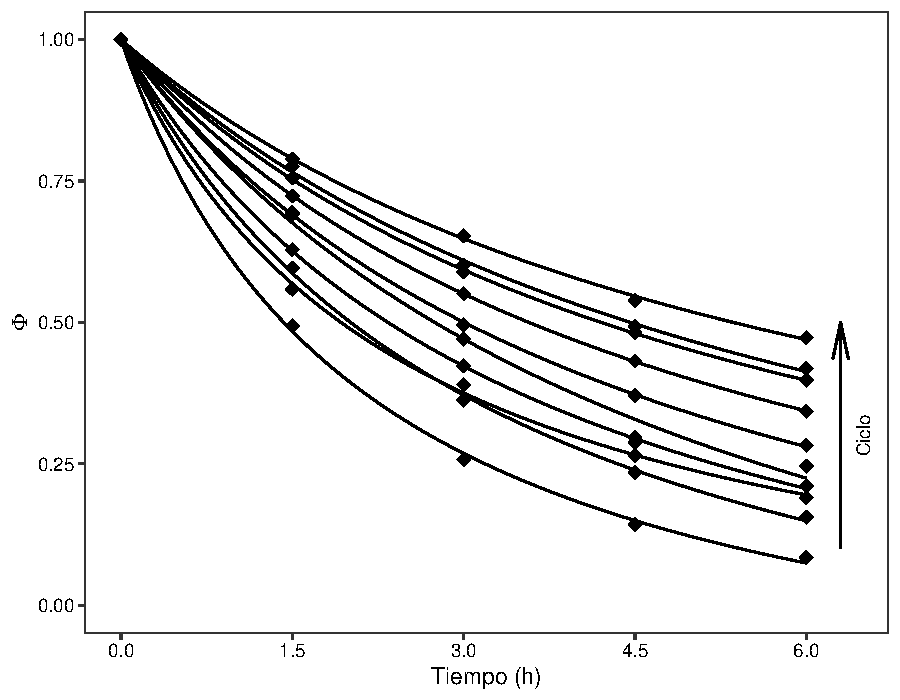
\includegraphics[height=0.388\textwidth]{chap5/figures/reuseprofiles.pdf}}
               \put(219, 168){\large a)}
               \end{picture}}%
    \subbottom{\begin{picture}(230,170)
               \put(0, 0){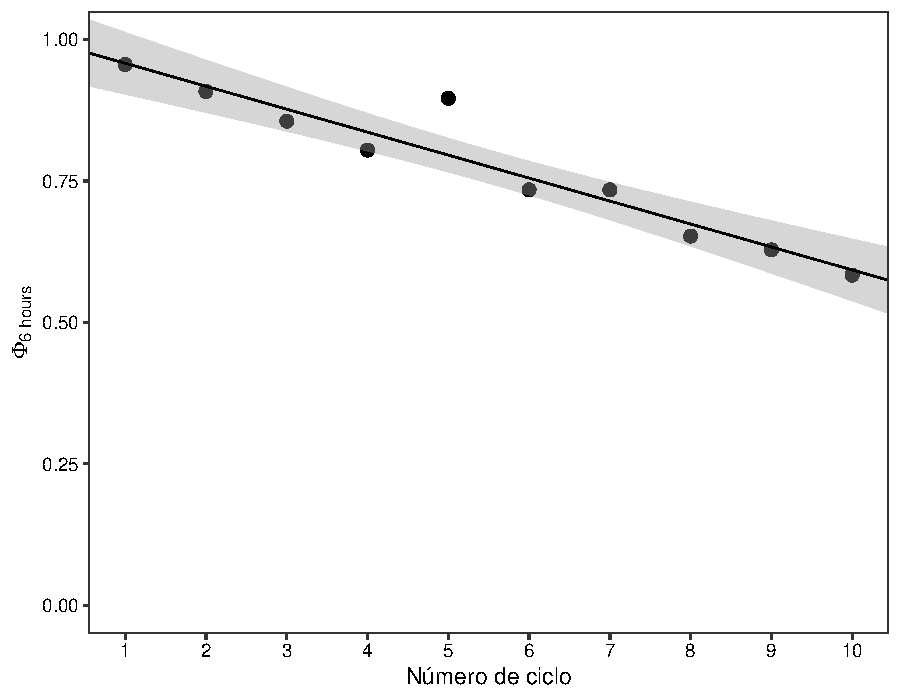
\includegraphics[height=0.388\textwidth, trim = {1.35cm 0 0 0},   clip]{chap5/figures/reusesummary.pdf}}
               \put(197, 168){\large b)}
               \end{picture}}\\
    \caption[Transporte de ion litio en varios ciclos reutilizando la membrana.]{Transporte de ion litio en varios ciclos reutilizando la membrana. (a) Perfiles de transporte desde la disolución de alimentación y (b) fracción transportada de ion litio hacia la disolución de recuperación tras seis horas en cada ciclo. La zona sombreada corresponde al intervalo de confianza de la regresión a un nivel de confianza del 95\%.}
    \label{fig:cycles}
\end{figure}

\subsection{Capacidad de concentración de ion litio}\label{sec:idealconc}
Con los resultados de secciones anteriores se conoció que el sistema es capaz de transportar ion litio en contra de su gradiente de concentración. Esto es posible si su transporte se acopla un contratransporte de iones hidronio. Tras la observación de que la membrana podía ser reutilizada para transportar ion litio se llevó a cabo un experimento similar en el que no se renovó la disolución de recuperación al final de cada ciclo con el propósito de obtener ion litio a una concentración mayor que la disponible inicialmente en la disolución de alimentación. El proceso de transporte se llevó a cabo bajo estas condiciones durante cinco ciclos y el perfil de transporte de ion litio se muestra en la Figura \ref{fig:liconc1}. 

El factor de concentración es de 3.2 luego de cinco ciclos de transporte de ion litio. Esto es equivalente a una eficiencia global de 64\%. Se observa que con cada cambio de la disolución de alimentación disminuye la eficiencia del proceso, como ya se había observado en la Sección \ref{sec:reuseres}. La concentración de ion litio es factible usando la metodología propuesta.

\begin{figure}[H]
    \centering
    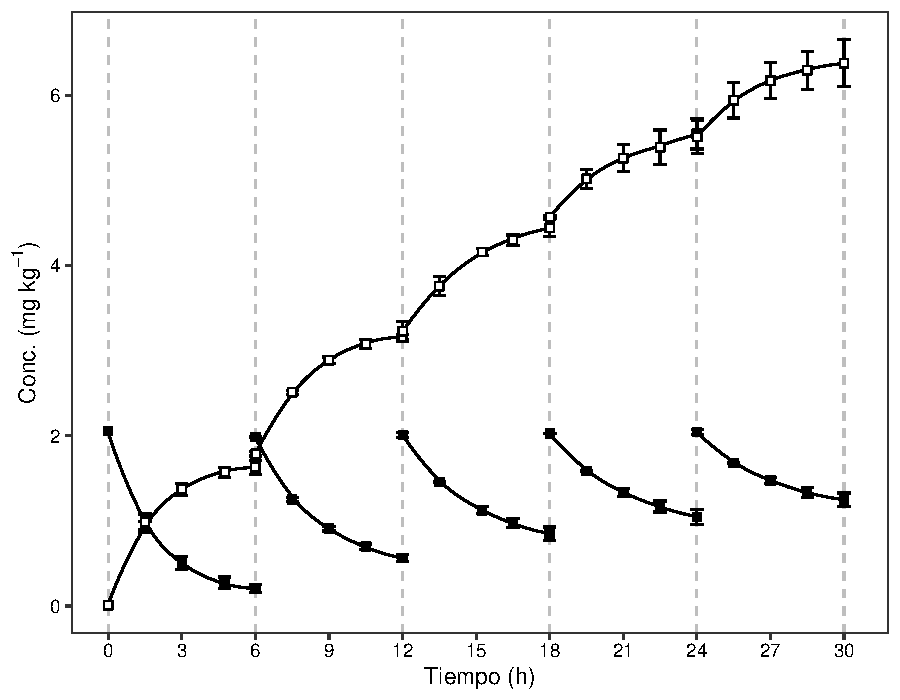
\includegraphics[width = 0.6\textwidth]{chap5/figures/liconc_0.pdf}
    \caption[Concentración de ion litio a partir de una disolución de alimentación ideal.]{Perfil de concentración de ion litio a partir de una disolución de alimentación ideal. Las líneas descontinuas verticales corresponden al inicio o al final de cada ciclo. (\protect\squareblck) ion litio en las disoluciones de alimentación y (\protect\squarewht) ion litio en la disolución de recuperación.}
    \label{fig:liconc1}
\end{figure}


\section{Agua de mar}\label{sec:resultsSSS}\index{Agua de mar}
Como ya se comentó en la Sección \ref{sec:selecresults}, el sistema no es selectivo frente al magnesio y probablemente tampoco lo sea frente al calcio. Estos cationes deben ser retirados del agua de mar antes de intentar extraer el ion litio. La relación molar \ce{Mg^2+}/\ce{Li+} y \ce{Ca^2+}/\ce{Li+} en agua de mar es de 2030:1 y 400:1, respectivamente \citep{Dickson1994}. La concentración final remanente de iones hidroxilo luego del proceso de precipitación por pasos usando hidróxido de sodio y monohidrógenofosfato de amonio se encuentra entre 0.03 y 0.04~mol~kg\mnn. La alcalinidad resultante del medio lo hace adecuado para su uso directo como disolución de alimentación sin la necesidad de añadir reactivos adicionales. 

El perfil de transporte de ion litio, sodio y potasio usando agua de mar sintética simplificada luego de la remoción de iones calcio y magnesio se muestra en la Figura \ref{fig:SSS1}(a). Los factores de separación de ion litio contra sodio y potasio se presentan en la  Figura \ref{fig:SSS1}(b).

El ion litio parece ser transportado en su totalidad hacia la disolución de recuperación tras 4.5 horas de iniciado el proceso. La concentración a la que se encuentra el ion litio en esta matriz es de 0.18~mg~kg\mnn, cerca de diez veces menor a la que contenía la disolución de alimentación con la que el proceso fue optimizado. Para un volumen constante, una menor concentración de ion litio en la disolución de alimentación hace que los cambios de esta magnitud en esta disolución como consecuencia del proceso de transporte, representen una proporción mayor de la especie presente al comienzo del experimento. Debido a esto, la depleción de iones litio de la disolución ocurre en un intervalo de tiempo más corto.  Por otro lado, debe considerarse que la concentración de iones sodio y potasio en el medio es muy alta. Aunque el sistema es muy selectivo frente a estos cationes, se demostró en la Figura \ref{fig:selectivity1} que cuando estas sustancias están a altas concentraciones, su cotransporte afecta de manera importante el transporte de ion litio.

\begin{figure}[H]
  \centering
    \subbottom{\begin{picture}(240,167)
               \put(0, 0){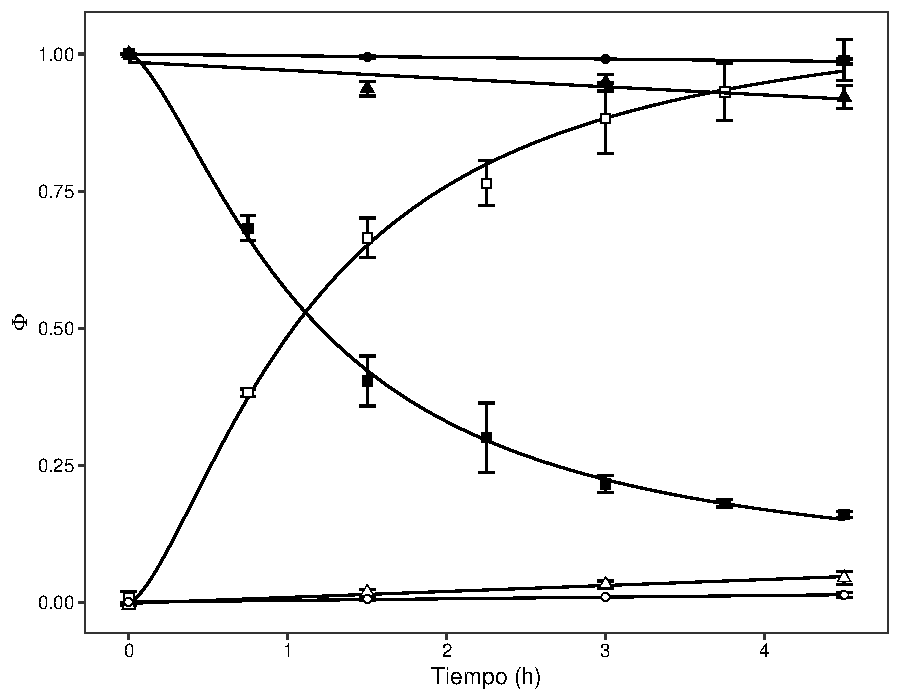
\includegraphics[height=0.37\textwidth, trim = {0cm 0 0 0},   clip]{chap5/figures/sssprof.pdf}}
               \put(-1, 161){\large a)}
               \end{picture}}%
    \subbottom{\begin{picture}(250,167)
               \put(0, 0){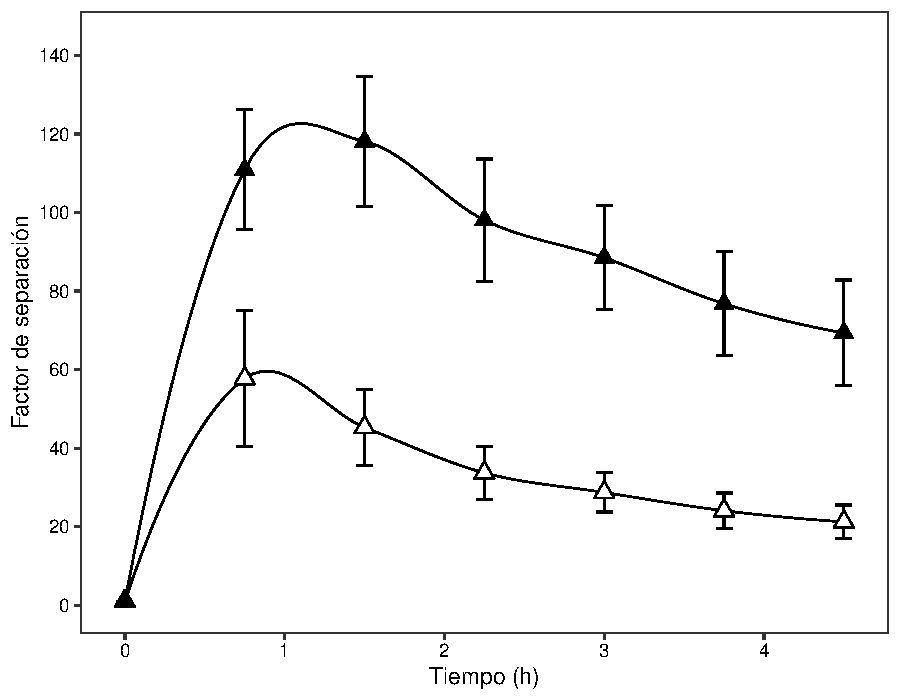
\includegraphics[height=0.37\textwidth, trim = {0cm 0 0 0},   clip]{chap5/figures/sssSep.pdf}}
               \put(-1, 161){\large b)}
               \end{picture}}\\
    \caption[Perfil de transporte y factores de separación usando agua de mar sintética simplificada.]{(a) Perfil de transporte usando agua de mar sintética simplificada: ion litio en la fase de alimentación (\protect\squareblck), ion litio en la fase de recuperación (\protect\squarewht), sodio en la fase de alimentación (\protect\triangleupblck), sodio en la fase de recuperación (\protect\triangleupwht), potasio en la fase de alimentación (\protect\circleblck) y potasio en la fase de recuperación (\protect\circlewht).  (b) factores de separación en función del tiempo: (\protect\triangleupblck) \ce{Li+}/\ce{K+} y (\protect\triangleupwht) \ce{Li+}/\ce{Na+}.}
  \label{fig:SSS1}
\end{figure}


En la Figura \ref{fig:SSS1}(a), la disolución de alimentación parece quedar hacia el final del proceso con un remanente del 15\% del ion litio presente inicialmente. Esto no concuerda con el perfil de transporte de ion litio hacia la disolución de recuperación en  donde aparentemente todo el ion litio es transportado al otro lado de la PIM. Esta posible inconsistencia en el balance de materia del sistema puede justificarse por un efecto matriz de naturaleza traslacional para la cuantificación de ion litio en la matriz de agua de mar. La cuantificación de ion litio se hizo por adición estándar de un punto (ver Anexo \ref{sec:quantification}) y esto mejoró significativamente el balance de materia para ion litio en las disoluciones corrigiendo los efectos matriz rotacionales debidos a los componentes presentes en el agua de mar. Sin embargo, la cuantificación por adición estándar de un solo punto es incapaz de corregir efectos matriz traslacionales \citep{Ellison2008}. Estos efectos matriz difíciles de corregir tienen un efecto más marcado a bajas concentraciones de ion litio. Es probable que en nuestro caso particular, el sesgo introducido cuando la concentración de ion litio es casi nula corresponda a una fracción de 0.15.

Los factores de separación máximos alcanzados frente a sodio y potasio son 118$\pm$16 y 57$\pm$17, respectivamente. Los factores de separación finales frente a sodio y potasio son 69$\pm$13 y 21$\pm$4, respectivamente. El sistema es capaz de selectivamente extraer ion litio de agua de mar.

\subsection{Muestras reales}
\subsubsection{Caracterización}
La concentración de iones litio, sodio, potasio, magnesio y calcio determinadas en las muestras de agua de mar natural recolectadas se muestra en la Tabla \ref{tab:swChar}
\begin{table}[H]
    \centering\footnotesize
    \begin{tabular}{@{}lccccc@{}}\toprule
        \multirow{2}{*}{\textbf{Procedencia}}&[\ce{Li^+}]&[\ce{Na^+}]&[\ce{K^+}]&[\ce{Mg^2+}]&[\ce{Ca^2+}]\\ 
        &(mg~kg\mnn)&(mg~kg\mnn)&(mg~kg\mnn)&(mg~kg\mnn)&(mg~kg\mnn)\\\midrule
        St.\ George Island, Estados Unidos &0.22$\pm$0.03 &~~9870$\pm$110 &359$\pm$22& 1173$\pm$32& 369$\pm$4\\[0.5ex]
        Santa Marta, Colombia &0.23$\pm$0.01 &10732$\pm$134 &401$\pm$10& 1278$\pm$33& 393$\pm$1\\[0.5ex]
        Referencia \citep{Trujillo2016} &0.18&10784&399&1284&415\\\bottomrule
    \end{tabular}
    \caption{Concentración de cationes en las muestras de agua de mar natural.}
    \label{tab:swChar}
\end{table}
La salinidad superficial del agua de mar tiende a ser mayor en inmediaciones a los Trópicos de Cáncer y Capricornio que en la Línea Ecuatorial \citep{Trujillo2016}. Esto se debe a una combinación de factores ambientales que favorecen la evaporación de agua en la zona de los trópicos aumentando la concentración de sales en el agua. La evaporación masiva de agua en la zona Ecuatorial también es un factor importante pero a diferencia de la zona de los Trópicos, la precipitación constante de agua fresca aminora el impacto que esto genera.

Contrario a lo descrito en el párrafo anterior, el agua proveniente de St.\ George Island, Estados Unidos, presenta una concentración menor de cationes respecto al agua muestreada en Santa Marta, Colombia. Esto puede atribuírse a que la isla se encuentra en la Bahía de Apalachicola, donde desemboca el agua dulce del Río Apalachicola. Este es el río más grande del Estado de Florida. El agua del río diluye levemente el agua salada que rodea la isla donde fue tomada la muestra de agua. Por otro lado, la única fuente de `agua dulce' cercana al punto de muestreo en Colombia es el Río Manzanares\footnote{El Río Manzanares sufre de un terrible daño ambiental por descarga de aguas residuales y de varias toneladas de basura al año \citep{Iguaran2019}. Lamentablemente, hace muchos años que sus aguas dejaron de ser \textit{dulces}.}. El caudal del Río Manzanares es pequeño y la Bahía de Santa Marta donde desemboca se encuentra más abierta al mar con lo que la dilución de las sales disueltas en el agua marina es mucho menor.

\subsubsection{Extracción y concentración de ion litio}

Las muestras procedentes de las dos locaciones fueron mezcladas y se removieron los iones calcio y magnesio por precipitación/centrifugación. Se llevaron a cabo cuatro ciclos de extracción de ion litio renovando la disolución de agua de mar en el compartimiento de alimentación. Cada ciclo tuvo una duración de 4.5 horas. 

La concentración de ion litio no es factible usando el sistema propuesto si no se reajusta la concentración de iones hidronio en la disolución de recuperación al final de cada ciclo de transporte. La acidez de la disolución de recuperación disminuye gradualmente y al volverse alcalina esta disolución, el transporte de ion litio no solo se detiene, sino que incluso es transportado de regreso hacia la disolución de alimentación como se muestra a partir del tercer ciclo en la Figura \ref{fig:FAIL}. 

\begin{figure}[H]
    \centering
    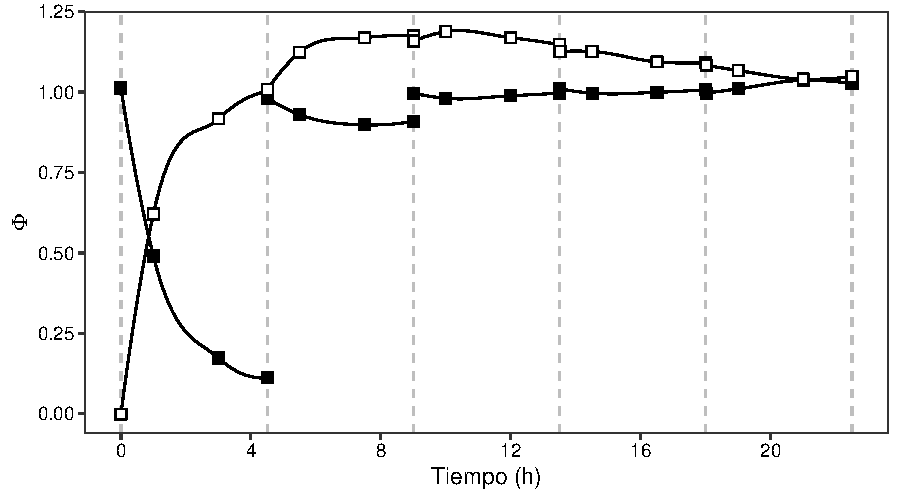
\includegraphics[width=0.65\textwidth, trim = {0cm 0 0 0},   clip]{chap5/figures/LiConcAS-FAIL.pdf}
    \caption[Concentración de ion litio sin reajustar la acidez en la fase de recuperación.]{Perfil de transporte de ion litio cuando se intenta concentrar a partir de agua de mar natural sin reajustar la concentración de iones hidronio en la disolución de recuperación al final de cada ciclo. (\protect\squareblck) ion litio en las disoluciones de alimentación y (\protect\squarewht) ion litio en la disolución de recuperación.}
    \label{fig:FAIL}
\end{figure}

La concentración de iones hidronio en la disolución de recuperación debe ser reajustada al valor original de 0.10~mol~kg\mnn\ al final de cada ciclo de extracción. La disminución en la concentración de iones hidronio en la fase de recuperación no fue importante cuando el ion litio se concentró a partir de una disolución de alimentación ideal. Cuando se usa agua de mar, el flujo de sodio y potasio hacia la disolución de recuperación es significativo a pesar de la buena selectividad del sistema. El flujo de cationes hacia la fase de recuperación conlleva un agotamiento de iones hidronio desde la misma. Si el flujo de cationes es significativo como en este caso, la disolución de recuperación puede volverse alcalina, y al desaparecer el gradiente de iones hidronio el transporte activo de iones litio se detiene. 

Se hizo un nuevo experimento reajustando la concentración de iones hidronio en la fase de recuperación al comienzo de cada ciclo. La concentración de iones litio, sodio, y potasio fue monitoreada en ambas disoluciones durante todo el proceso y los perfiles de transporte obtenidos se muestran en la Figura \ref{fig:liconcSW}. Puede observarse que reajustar la concentración de iones hidronio al final de cada ciclo parece ser suficiente para lograr la concentración de ion litio. Otra alternativa pudo haber sido mantener constante la acidez de esta disolución, por medio de la adición de sustancias amortiguadoras de pH. Esta opción no fue evaluada porque se deseó mantener la matriz de la disolución de alimentación tan simple como fuese posible.

\begin{figure}[htbp]
    \centering
    \subbottom{\begin{picture}(330,145)
               \put(0, 0){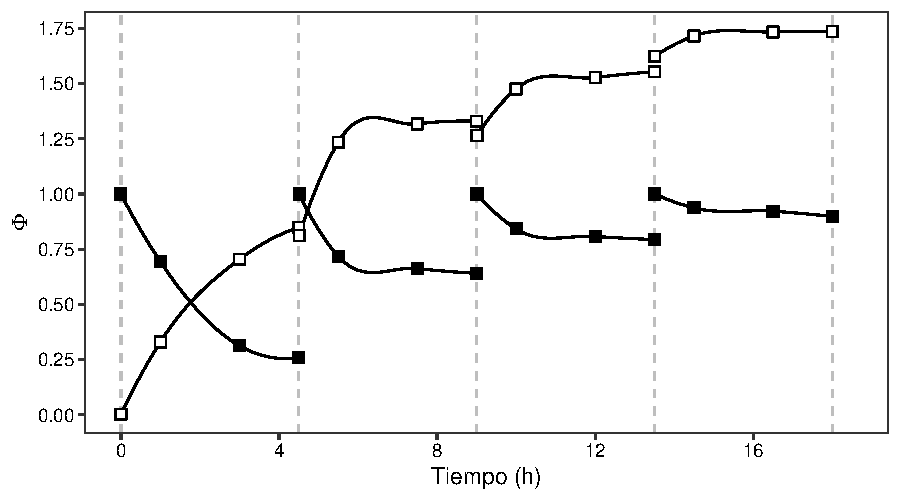
\includegraphics[width=0.65\textwidth, trim = {0cm 0.96cm 0 0},   clip]{chap5/figures/LiConcAS.pdf}}
               \put(-1, 137){\large a)}
               \end{picture}}\\
    \subbottom{\begin{picture}(330,145)
               \put(0, 0){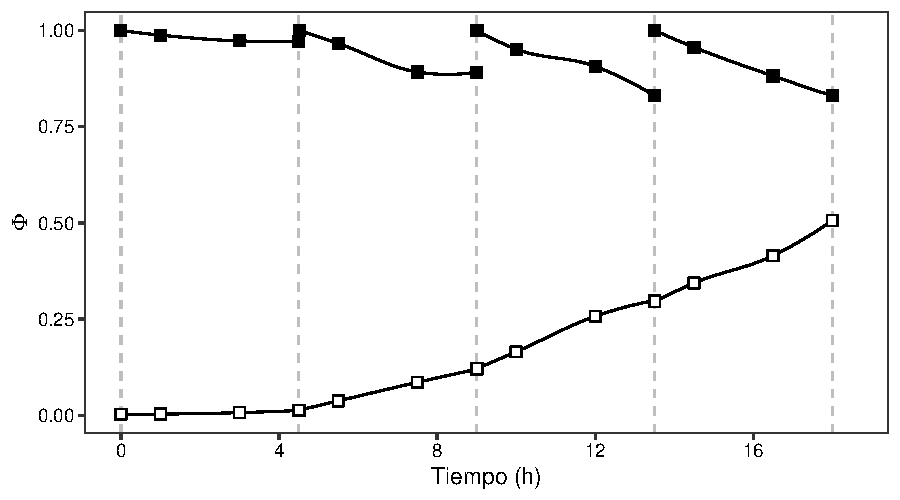
\includegraphics[width=0.65\textwidth, trim = {0cm 0.96cm 0 0},   clip]{chap5/figures/NaConcAS.pdf}}
               \put(-1, 137){\large b)}
               \end{picture}}\\
    \subbottom{\begin{picture}(330,165)
               \put(0, 0){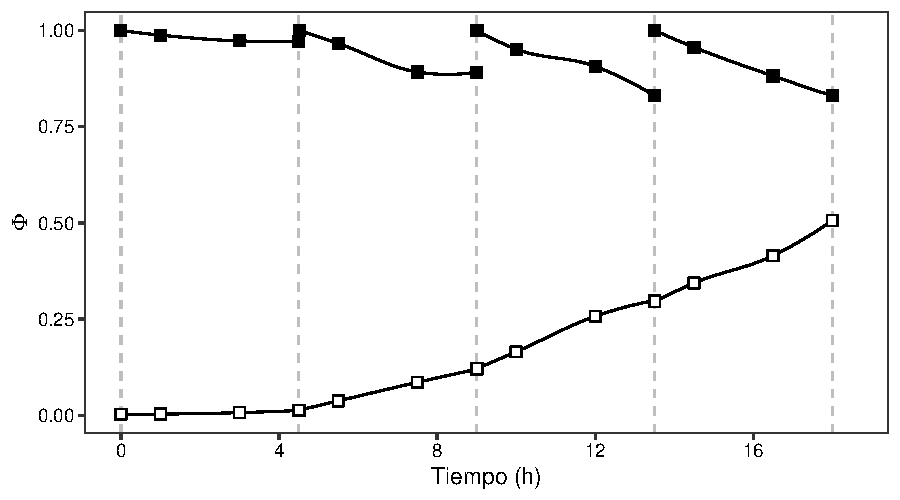
\includegraphics[width=0.65\textwidth, trim = {0cm 0 0 0},   clip]{chap5/figures/KConcAS.pdf}}
               \put(-1, 155){\large c)}
               \end{picture}}
    \caption[Concentración selectiva de ion litio a partir de agua de mar natural.]{Perfil de transporte de ion litio (a), ion sodio (b), e ion potasio (c) a partir de agua de mar natural sin calcio ni magnesio. Las líneas descontinuas verticales corresponden al inicio o al final de cada ciclo. (\protect\squareblck) especie en las disoluciones de alimentación y (\protect\squarewht) especie en la disolución de recuperación.}
    \label{fig:liconcSW}
\end{figure}

La capacidad de la membrana para extraer ion litio se ve deteriorada tras cada ciclo. El perfil de transporte para la concentración de ion litio usando agua de mar (Figura \ref{fig:liconcSW}(a)) difiere significativamente del obtenido cuando se usa una disolución de alimentación sin interferentes (Figura \ref{fig:liconc1}). Al usar una disolución de alimentación ideal, las pérdidas en la eficiencia del transporte disminuyen sutilmente tras cada ciclo y la membrana opera casi al 50\% de su capacidad en el quinto ciclo de concentración. Cuando se usa agua de mar, la eficiencia del sistema en el segundo ciclo es la mitad de la obtenida en el primer ciclo. En el cuarto ciclo la cantidad de ion litio extraído es solo el 13\% del que se extrae en el primer ciclo.

Un comportamiento muy diferente se observa para los cationes interferentes sodio y potasio. La fracción extraída de estos iones al final de cada ciclo es cada vez mayor. Excluyendo los cationes divalentes, la selectividad del sistema es \ce{Li+} $\gg$ \ce{Na+} > \ce{K+} (ver Sección \ref{sec:selecresults}). A partir del segundo ciclo, el orden entre sodio y potasio se invierte y el sistema empieza a extraer potasio con mayor eficiencia que con la que extrae sodio. En el cuarto ciclo la fracción de potasio que es transportada desde la disolución de alimentación es mayor a la de ion litio en casi un 10\%. Esto se presenta a pesar de que el potasio se encuentra en un exceso molar respecto al ion litio de casi 400:1. La selectividad del sistema para extraer ion litio se pierde en este punto y el nuevo orden de afinidad de la membrana pasa a ser \ce{K+} > \ce{Li+} > \ce{Na+}. Los factores de separación de ion litio respecto a sodio y potasio en función del tiempo se muestran en la Figura \ref{fig:SWselec}. Los valores finales de estos factores son 4.9 y 3.4, respectivamente. Los datos del primer ciclo caen en el intervalo de los obtenidos para el mismo experimento cuando la extracción selectiva de ion litio se hizo a partir de la receta de agua de mar sintética simplificada (Figura \ref{fig:SSS1}(b))

\begin{figure}[H]
    \centering
    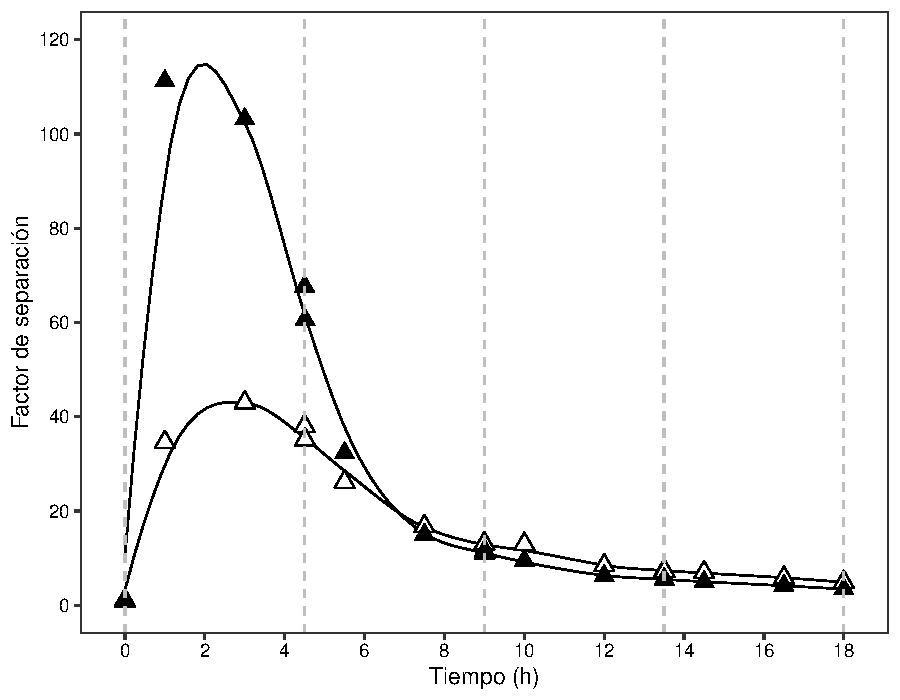
\includegraphics[width=0.6\textwidth, trim = {0cm 0cm 0 0}, clip]{chap5/figures/SW_Sep.pdf}
    \caption[Factor de separación de ion litio frente a sodio y potasio usando agua de mar natural.]{Factores de separación en función del tiempo para la concentración de ion litio usando agua de mar natural: (\protect\triangleupblck) \ce{Li+}/\ce{K+} y (\protect\triangleupwht) \ce{Li+}/\ce{Na+}. Las líneas descontinuas verticales corresponden al inicio o al final de cada ciclo.}
    \label{fig:SWselec}
\end{figure}

El factor de concentración de ion litio en agua de mar es 1.73 luego de cuatro ciclos de extracción. La eficiencia general de este proceso es de al rededor del 43\%, significativamente menor a la reportada en la Sección \ref{sec:idealconc} (64\%).

